\documentclass[a4paper,12pt]{extarticle}
\usepackage[utf8x]{inputenc}
\usepackage[T1,T2A]{fontenc}
\usepackage[russian]{babel}
\usepackage{hyperref}
\usepackage{indentfirst}
\usepackage{listings}
\usepackage{color}
\usepackage{here}
\usepackage{array}
\usepackage{multirow}
\usepackage{graphicx}

\usepackage{amsmath}

\usepackage{caption}
\renewcommand{\lstlistingname}{Программа} % заголовок листингов кода

\bibliographystyle{ugost2008ls}

\usepackage{listings}
\lstset{ %
extendedchars=\true,
keepspaces=true,
language=C,						% choose the language of the code
basicstyle=\footnotesize,		% the size of the fonts that are used for the code
numbers=left,					% where to put the line-numbers
numberstyle=\footnotesize,		% the size of the fonts that are used for the line-numbers
stepnumber=1,					% the step between two line-numbers. If it is 1 each line will be numbered
numbersep=5pt,					% how far the line-numbers are from the code
backgroundcolor=\color{white},	% choose the background color. You must add \usepackage{color}
showspaces=false				% show spaces adding particular underscores
showstringspaces=false,			% underline spaces within strings
showtabs=false,					% show tabs within strings adding particular underscores
frame=single,           		% adds a frame around the code
tabsize=2,						% sets default tabsize to 2 spaces
captionpos=t,					% sets the caption-position to top
breaklines=true,				% sets automatic line breaking
breakatwhitespace=false,		% sets if automatic breaks should only happen at whitespace
escapeinside={\%*}{*)},			% if you want to add a comment within your code
postbreak=\raisebox{0ex}[0ex][0ex]{\ensuremath{\color{red}\hookrightarrow\space}},
texcl=true,
inputpath=listings,                     % директория с листингами
}

\usepackage[left=2cm,right=2cm,
top=2cm,bottom=2cm,bindingoffset=0cm]{geometry}

%% Нумерация картинок по секциям
\usepackage{chngcntr}
\counterwithin{figure}{section}
\counterwithin{table}{section}

%%Точки нумерации заголовков
\usepackage{titlesec}
\titlelabel{\thetitle.\quad}
\usepackage[dotinlabels]{titletoc}

%% Оформления подписи рисунка
\addto\captionsrussian{\renewcommand{\figurename}{Рисунок}}
\captionsetup[figure]{labelsep = period}

%% Подпись таблицы
\DeclareCaptionFormat{hfillstart}{\hfill#1#2#3\par}
\captionsetup[table]{format=hfillstart,labelsep=newline,justification=centering,skip=-10pt,textfont=bf}

%% Путь к каталогу с рисунками
\graphicspath{{fig/}}


\setcounter{tocdepth}{3}

\begin{document}	% начало документа

% Титульная страница
\begin{titlepage}	% начало титульной страницы

	\begin{center}		% выравнивание по центру

		\large Санкт-Петербургский Политехнический Университет Петра Великого\\
		\large Институт компьютерных наук и технологий \\
		\large Кафедра компьютерных систем и программных технологий\\[6cm]
		% название института, затем отступ 6см
		
		\huge Телекоммуникационные технологии\\[0.5cm] % название работы, затем отступ 0,5см
		\large Отчет по лабораторной работе №4\\[0.1cm]
		\large Аналоговая модуляция\\[5cm]

	\end{center}


	\begin{flushright} % выравнивание по правому краю
		\begin{minipage}{0.25\textwidth} % врезка в половину ширины текста
			\begin{flushleft} % выровнять её содержимое по левому краю

				\large\textbf{Работу выполнил:}\\
				\large Соболь В.О.\\
				\large {Группа:} 33501/4\\
				
				\large \textbf{Преподаватель:}\\
				\large Богач Н.В.

			\end{flushleft}
		\end{minipage}
	\end{flushright}
	
	\vfill % заполнить всё доступное ниже пространство

	\begin{center}
	\large Санкт-Петербург\\
	\large \the\year % вывести дату
	\end{center} % закончить выравнивание по центру

\thispagestyle{empty} % не нумеровать страницу
\end{titlepage} % конец титульной страницы

\vfill % заполнить всё доступное ниже пространство

% Содержание
% Содержание
\renewcommand\contentsname{\centerline{Содержание}}
\tableofcontents
\newpage



 
\section{Цель работы}
Изучение различных методов модуляции цифровых сигналов.
 
\section{Постановка задачи}
В ходе работы необходимо получить различные сигналы используя BPSK, PSK, OQPSK, genQAM, MSK, M-FSK модуляторы.
Также необходимо построить сигнальные созвездия и провести сравнение изученных методов модуляции цифровых сигналов.

\section{Теоретическая информация}

\subsection{Типы цифровой модуляции}

Цифровая модуляция и демодуляция включают в себя две стадии. При модуляции цифровое сообщение сначала преобразуется в аналоговый модулирующий сигнал, а затем осуществляется аналоговая модуляция. При демодуляции сначала получается аналоговый демодулированный сигнал, а затем он преобразуется в цифровое сообщение.
 
Аналоговый несущий сигнал модулируется цифровым битовым потоком.
Существуют четыре типа цифровой модуляции:
\begin{enumerate}
\item ASK – Amplitude shift keying (Амплитудная двоичная модуляция).
\item FSK – Frequency shift keying (Частотная двоичная модуляция).
\item PSK – Phase shift keying (Фазовая двоичная модуляция).
\item ASK/PSK.
\end{enumerate}
Одна из частных реализаций схемы ASK/PSK - QAM - Quadrature Amplitude Modulation (квадратурная амплитудная модуляция).
Это метод объединения двух AM-сигналов в одном канале. Он позволяет удвоить эффективную пропускную способность.
В QAM используется две несущих с одинаковой частотой но с разницей в фазе на четверть периода.

Частотная модуляция представляет логическую единицу интервалом с большей частотой, чем ноль.
Фазовый сдвиг представляет ''0'' как сигнал без сдвига, а ''1'' как сигнал со сдвигом.
BPSK использует единственный сдвиг фазы между ''0'' и ''1'' — 180 градусов, половина периода.
QPSK использует 4 различных сдвига фазы (по четверти периода) и может кодировать 2 бита в символе (01, 11, 00, 10).

\subsubsection{BPSK, PSK}
BPSK и PSK - модуляция со сдвиглм фазы сигнала без изменения амплитуды. В PSK их может быть множество, в BPSK - один 
(на $\pi$).

Изображения сигнального созвездия BPSK приведено на следующих рис.~\ref{BPSK_Sig_Con_theor}.

\begin{figure}[H]
	\begin{center}
		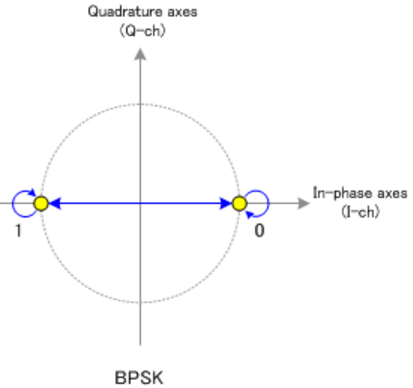
\includegraphics[width=\textwidth]{BPSK_Sig_Con_theor.png}
		\caption{Сигнальное созвездие BPSK.} %% подпись к рисунку
		\label{BPSK_Sig_Con_theor} %% метка рисунка для ссылки на него
	\end{center}
\end{figure}

\subsubsection{genQAM, OQPSK}
При квадратурной амплитудной модуляции изменяется как фаза, так и амплитуда несущего сигнала.
 Это позволяет увеличить количество кодируемых в единицу времени бит и при этом повысить помехоустойчивость их передачи по каналу связи. Квадратурное представление сигнала заключается в выражении колебания линейной комбинацией двух ортогональных составляющих – квадратурной и синфазной:
\begin{equation}
	S(t) = x(t) sin(\omega t + \varphi) cos(\omega t + \varphi)
\end{equation}
где $x(t)$ и $y(t)$ – биполярные дискретные сигналы.

Модуляция со сдвигом (OQPSK – Offset QPSK) позволяет избежать скачков фазы на $180^0$ и, следовательно, глубокой модуляции
 огибающей. Формирование сигнала в модуляторе OQPSK происходит так же, как и в модуляторе ФМ-4, за исключением того, что
  манипуляционные элементы информационных последовательностей $x(t)$ и $y(t)$ смещены во времени на длительность одного 
  элемента $Т$, (рис.\ref{manip_sig_theor}). Изменение фазы при таком смещении модулирующих потоков определяется лишь одним 
  элементом последовательности, а не двумя, как при ФМ 4. В результате скачки фазы на $180^0$ отсутствуют, так как каждый 
  элемент последовательности, поступающий на вход модулятора синфазного или квадратурного канала, может вызвать изменение 
  фазы на $0$, $+90°$ или $-90°$.
\begin{figure}[H]
	\begin{center}
		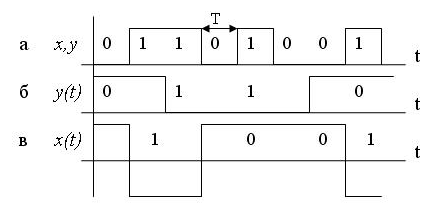
\includegraphics[width=\textwidth]{manip_sig_theor.png}
		\caption{Формирование манипулирующих сигналов} %% подпись к рисунку
		\label{manip_sig_theor} %% метка рисунка для ссылки на него
	\end{center}
\end{figure} 

Преобразованные таким образом сигналы передаются в одном канале. Поскольку один и тот же физический канал используется для передачи двух сигналов, то скорость передачи КАМ-сигнала в отличие от АМ-сигнала в два раза выше.


\subsubsection{MSK}
Частотная манипуляция с минимальным сдвигом (англ. Minimal Shift Keying (MSK)) представляет собой способ модуляции, при котором не происходит скачков фазы и изменение частоты происходит в моменты пересечения несущей нулевого уровня.
 MSK характеризуется тем, что значение частот соответствующих логическим ''0'' и ''1'' отличаются на величину равную половине скорости передачи данных. Другими словами, индекс модуляции равен $0.5$.

Изображение сигнального созвездия MSK приведено рис.~\ref{MSK_sig_con_theor}.

\begin{figure}[H]
	\begin{center}
		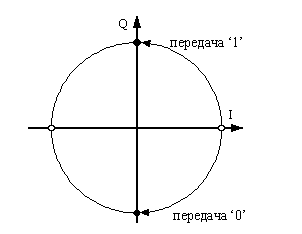
\includegraphics[width=\textwidth]{MSK_sig_con_theor.png}
		\caption{Сигнальное созвездие MSK.} %% подпись к рисунку
		\label{MSK_sig_con_theor} %% метка рисунка для ссылки на него
	\end{center}
\end{figure}

\subsubsection{MFSK}
Можно построить и модулятор многопозиционной частотной модуляции. В этом случае будет использовано большее количество синусоидальных генераторов, а для управления коммутатором потребуется многоразрядное двоичное число.

Сигналы в многопозиционной частотной модуляции могут быть описаны в соответствии со следующим выражением:
\begin{equation}
	s_1 (t) =  cos(\omega_1 t); s_2 (t) =  cos(\omega_2 t); ...; s_N (t) =  cos(\omega_N t); 
\end{equation}
формула сигнала 1 многопозиционной частотной модуляции,  формула сигнала 2 многопозиционной частотной модуляции, …,  формула сигнала N многопозиционной частотной модуляции (3)
где $s_1$ используется для передачи первого состояния символа;
$s_2$ — для передачи второго состояния символа;
$s_N$ — для передачи N-го состояния символа.

Использование многопозиционной частотной модуляции позволяет реализовать высокочастотный сигнал с постоянной амплитудой. Такой сигнал позволяет строить радиопередатчики с максимальным кпд, так как при применении сигнала с постоянной амплитудой, усилитель мощности радиопередатчика работает в оптимальном режиме.

\section{Ход работы}

В ходе работы были получены модуляции: BPSK, PSK, OQPSK, genQAM, MSK и MFSK.
Результаты приведены ниже.

\subsection{BPSK-модуляция}

BPSK модуляция получена с помощью кода из листинга~\ref{code:code}. 
Исходный сигнал и демодулированный показаны на рис.~\ref{signal_BPSK}. Сигнальное созвездие
модулированного сигнала показано на рис.~\ref{scatter_BPSK}.

\begin{figure}[H]
	\begin{center}
		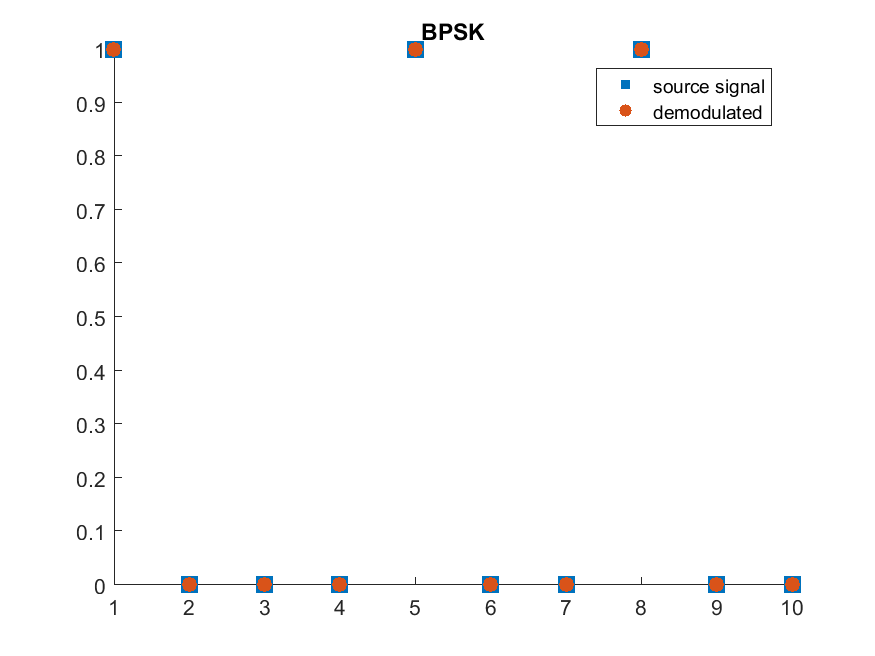
\includegraphics[width=\textwidth]{signal_BPSK.png}
		\caption{сигналы} %% подпись к рисунку
		\label{signal_BPSK} %% метка рисунка для ссылки на него
	\end{center}
\end{figure}

\begin{figure}[H]
	\begin{center}
		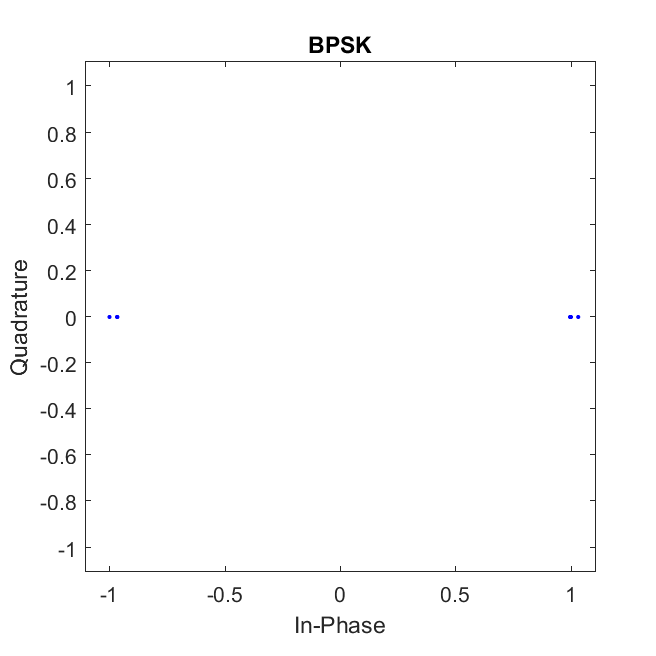
\includegraphics[width=\textwidth]{scatter_BPSK.png}
		\caption{Сигнальное созвездие} %% подпись к рисунку
		\label{scatter_BPSK} %% метка рисунка для ссылки на него
	\end{center}
\end{figure}

Видно, что демодулированный сигнал совпал с исходным.

\subsection{PSK-модуляция}
 
PSK модуляция получена с помощью кода из листинга~\ref{code:code}. 
Исходный сигнал и демодулированный показаны на рис.~\ref{signal_PSK}. Сигнальное созвездие
модулированного сигнала показано на рис.~\ref{scatter_PSK}.
\begin{figure}[H]
	\begin{center}
		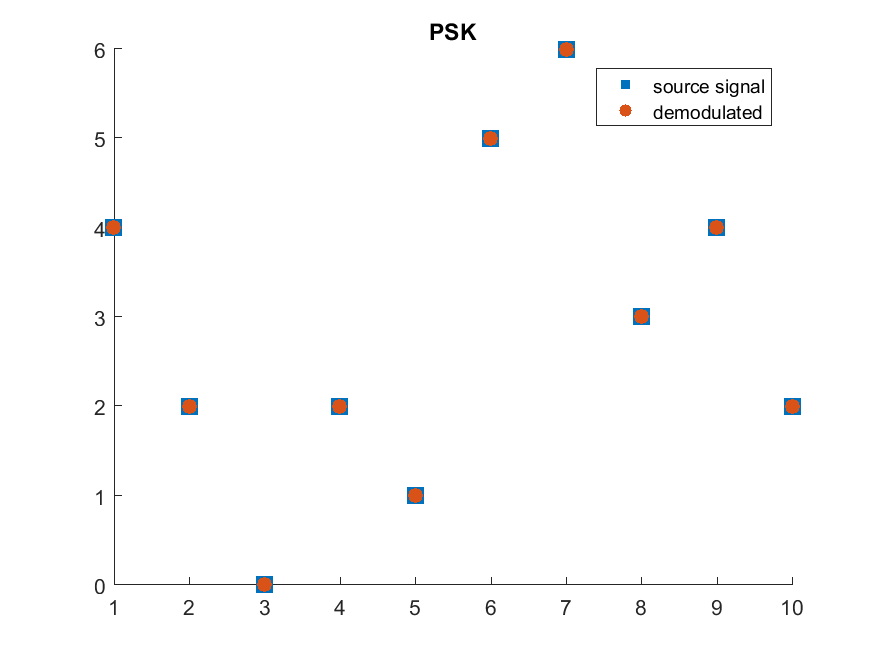
\includegraphics[width=\textwidth]{signal_PSK.png}
		\caption{сигналы} %% подпись к рисунку
		\label{signal_PSK} %% метка рисунка для ссылки на него
	\end{center}
\end{figure}

\begin{figure}[H]
	\begin{center}
		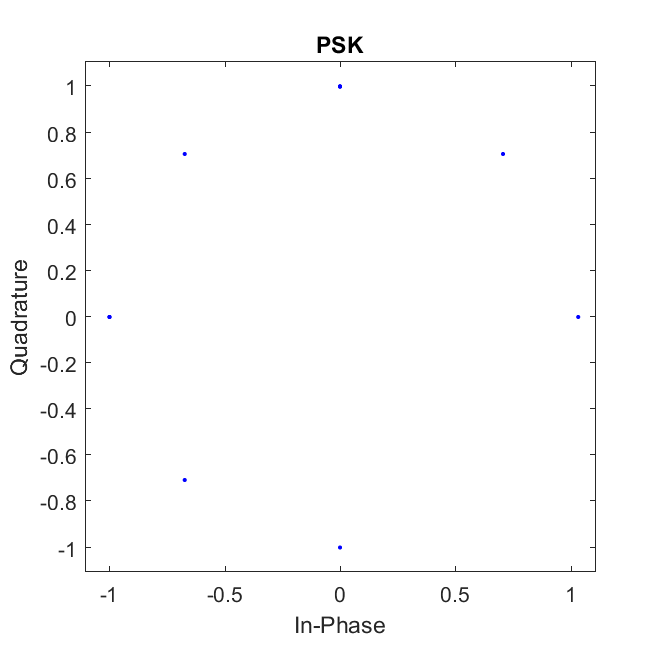
\includegraphics[width=\textwidth]{scatter_PSK.png}
		\caption{Сигнальное созвездие} %% подпись к рисунку
		\label{scatter_PSK} %% метка рисунка для ссылки на него
	\end{center}
\end{figure}

Видно, что демодулированный сигнал совпал с исходным.


\subsection{OQPSK-модуляция}

OQPSK модуляция получена с помощью кода из листинга~\ref{code:code}. 
Исходный сигнал и демодулированный показаны на рис.~\ref{signal_OQPSK}. Сигнальное созвездие
модулированного сигнала показано на рис.~\ref{scatter_OQPSK}.
\begin{figure}[H]
	\begin{center}
		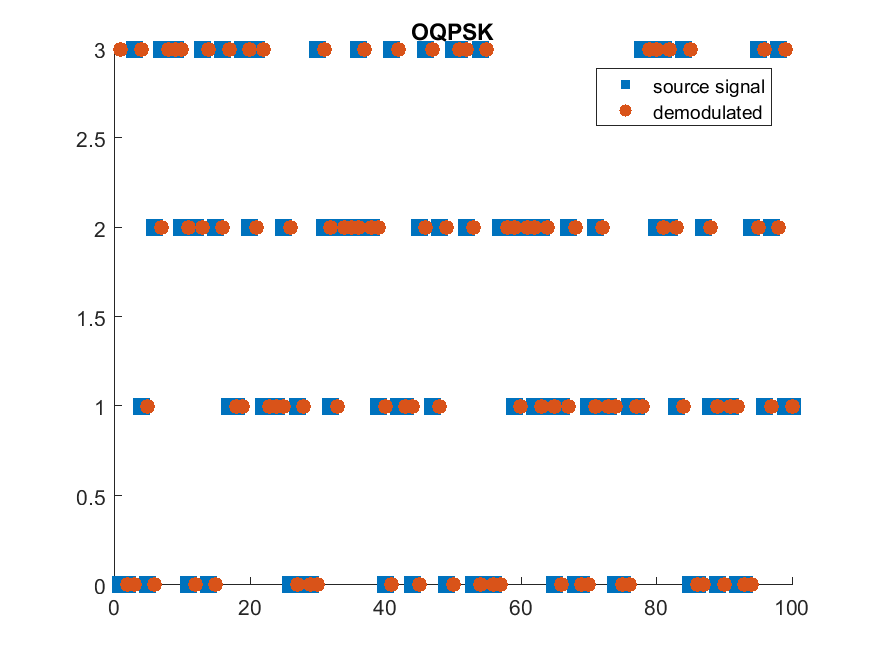
\includegraphics[width=\textwidth]{signal_OQPSK.png}
		\caption{сигналы} %% подпись к рисунку
		\label{signal_OQPSK} %% метка рисунка для ссылки на него
	\end{center}
\end{figure}

\begin{figure}[H]
	\begin{center}
		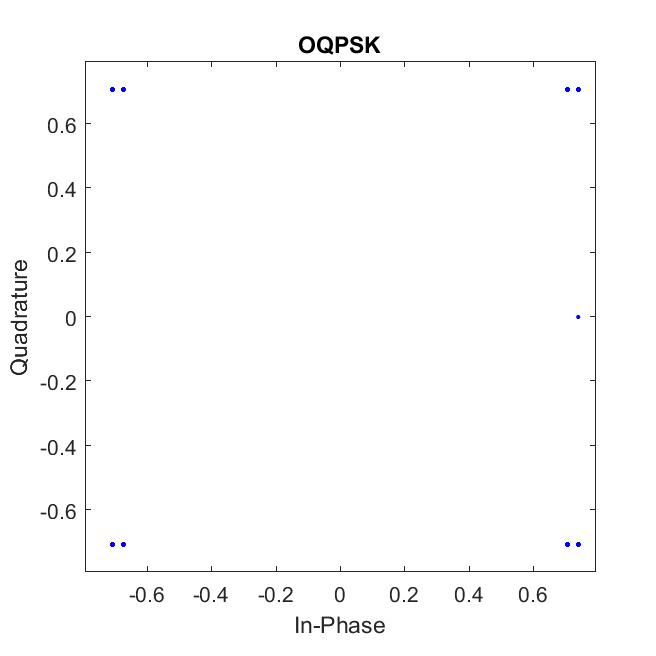
\includegraphics[width=\textwidth]{scatter_OQPSK.png}
		\caption{Сигнальное созвездие} %% подпись к рисунку
		\label{scatter_OQPSK} %% метка рисунка для ссылки на него
	\end{center}
\end{figure}

Видно, что демодулированный сигнал совпал с исходным.

\subsection{genQAM-модуляция}

Gen QAM модуляция получена с помощью кода из листинга~\ref{code:code}. 
Исходный сигнал и демодулированный показаны на рис.~\ref{signal_genQAM}. Сигнальное созвездие
модулированного сигнала показано на рис.~\ref{scatter_genQAM}.
\begin{figure}[H]
	\begin{center}
		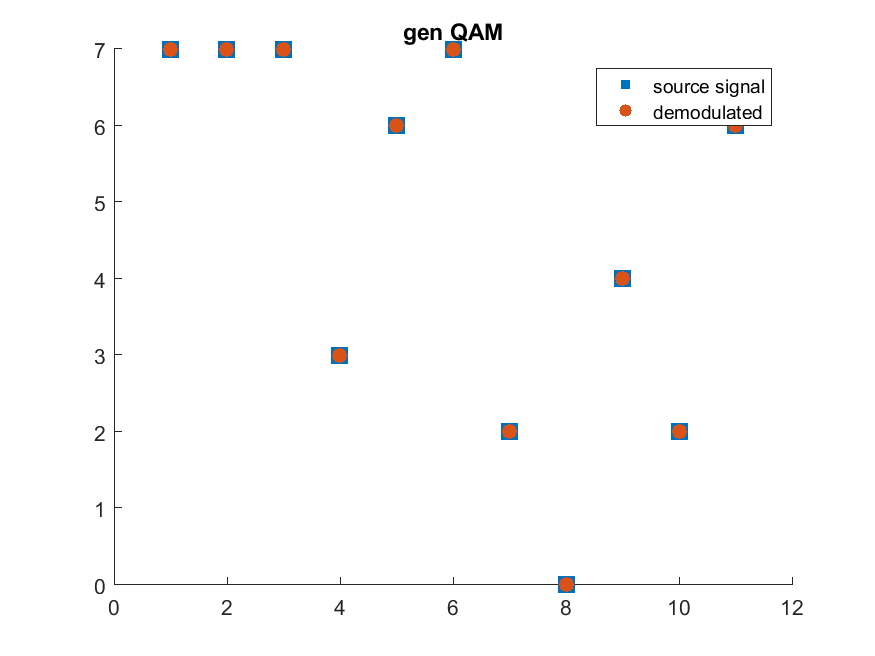
\includegraphics[width=\textwidth]{signal_genQAM.png}
		\caption{сигналы} %% подпись к рисунку
		\label{signal_genQAM} %% метка рисунка для ссылки на него
	\end{center}
\end{figure}

\begin{figure}[H]
	\begin{center}
		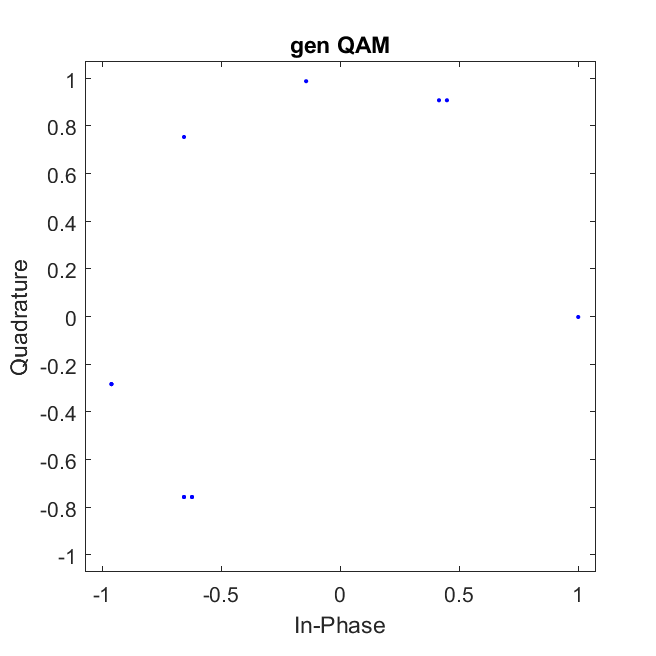
\includegraphics[width=\textwidth]{scatter_genQAM.png}
		\caption{Сигнальное созвездие} %% подпись к рисунку
		\label{scatter_genQAM} %% метка рисунка для ссылки на него
	\end{center}
\end{figure}

Видно, что демодулированный сигнал совпал с исходным.

\subsection{MSK-модуляция}

MSK модуляция получена с помощью кода из листинга~\ref{code:code}. 
Исходный сигнал и демодулированный показаны на рис.~\ref{signal_msk}. Сигнальное созвездие
модулированного сигнала показано на рис.~\ref{scatter_msk}.
\begin{figure}[H]
	\begin{center}
		\includegraphics[width=\textwidth]{signal_msk.png}
		\caption{сигналы} %% подпись к рисунку
		\label{signal_msk} %% метка рисунка для ссылки на него
	\end{center}
\end{figure}

\begin{figure}[H]
	\begin{center}
		\includegraphics[width=\textwidth]{scatter_msk.png}
		\caption{Сигнальное созвездие} %% подпись к рисунку
		\label{scatter_msk} %% метка рисунка для ссылки на него
	\end{center}
\end{figure}

Как можно видеть, при использовании MSK выходной сигнал имеет задержку при демодуляции.
Видно, что демодулированный сигнал совпал с исходным.


\subsection{MFSK-модуляция}

В Simulink была построена модель MFSK-модулятора, результаты работы совпали с ожидаемыми, входная последовательность совпала с выходной.
\begin{figure}[H]
	\begin{center}
		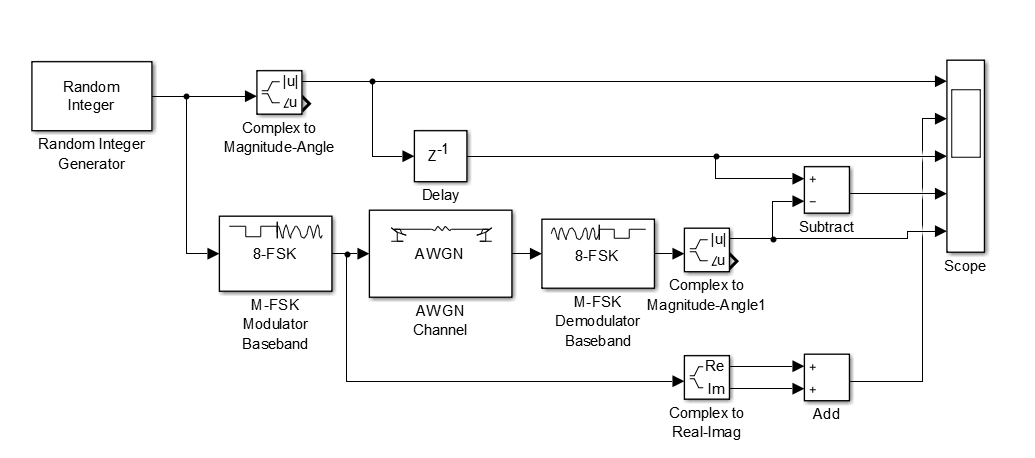
\includegraphics[width=\textwidth]{MFSK_Mod_theor.png}
		\caption{Simulink-модель MFSK.} %% подпись к рисунку
		\label{MFSK_Mod_theor} %% метка рисунка для ссылки на него
	\end{center}
\end{figure}

\begin{figure}[H]
	\begin{center}
		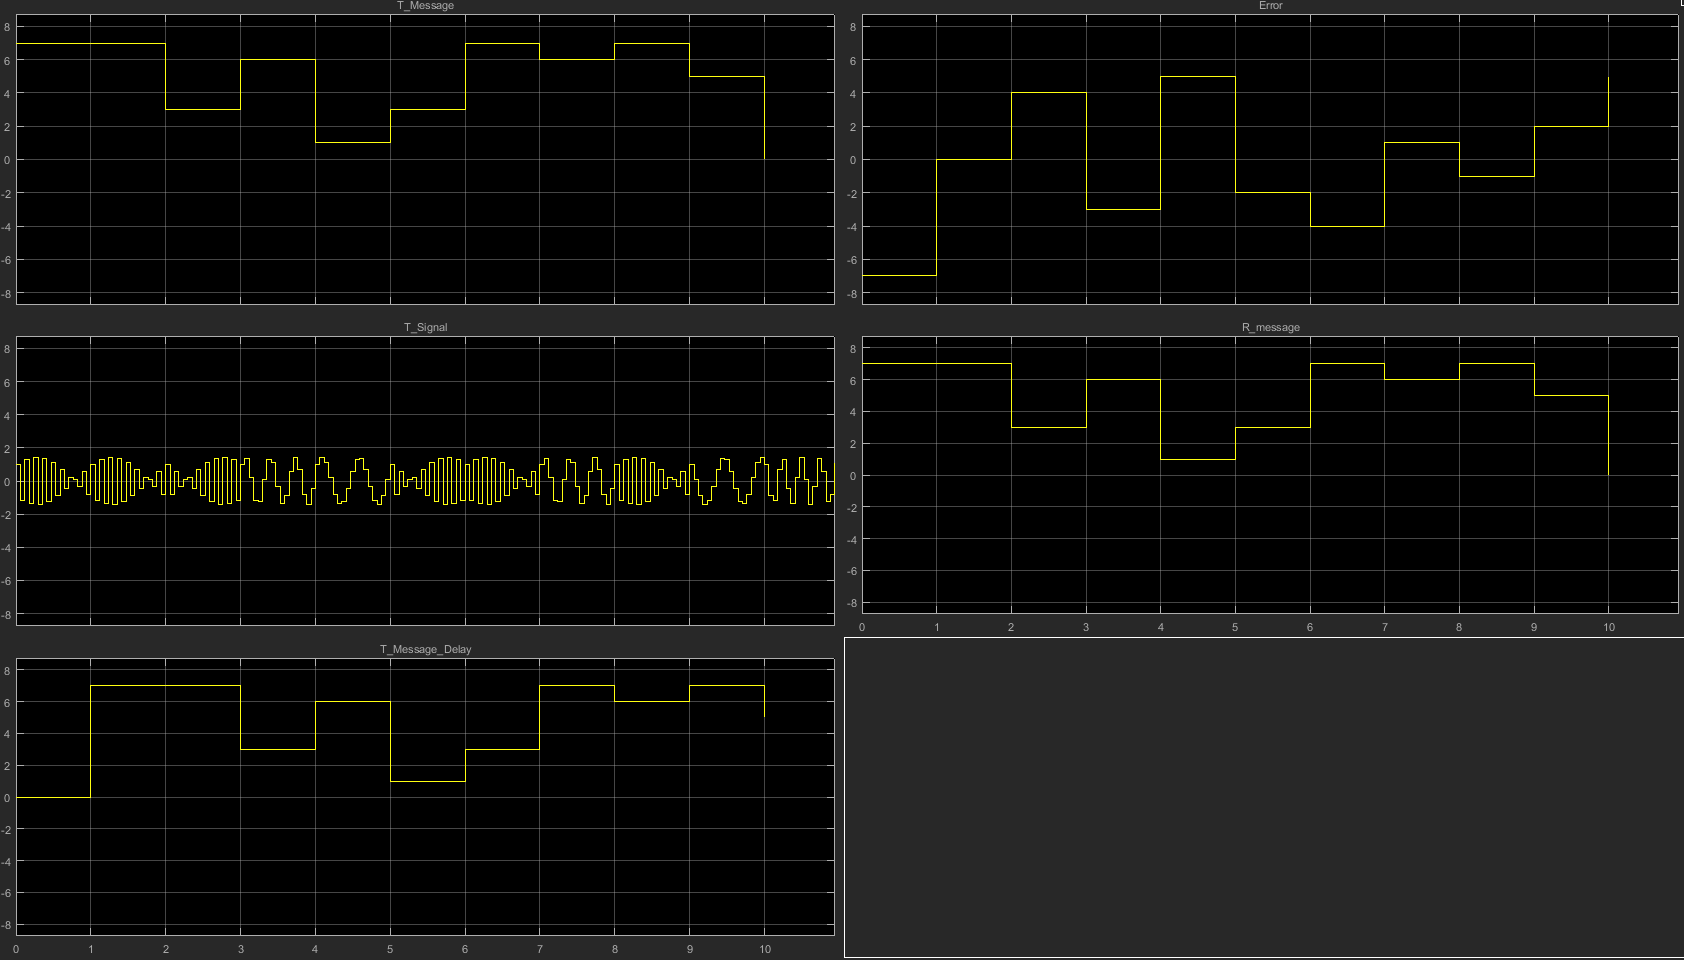
\includegraphics[width=\textwidth]{MFSK_Gen.png}
		\caption{Графики входного сигнала, задержанного сигнала, модулированного сигнала, сигнала ошибки с задержанным сигналом, выходного сигнала MFSK.} %% подпись к рисунку
		\label{MFSK_Gen} %% метка рисунка для ссылки на него
	\end{center}
\end{figure}
  
 
\section{Выводы}

Квадратурная амплитудная манипуляция (QAM) — манипуляция, при которой изменяется как фаза, так и амплитуда сигнала, что позволяет увеличить количество информации, передаваемой одним состоянием сигнала. 

Фазовая манипуляция (PSK) — модуляция, при которой фаза несущего колебания меняется скачкообразно. 

При квадратурной фазовой манипуляции (QPSK) используется созвездие из четырёх точек, размещённых на равных расстояниях на окружности. Имеется 4 фазовых смещения, при этом в QPSK на символ приходится два бита. 

Частотная манипуляция с минимальным сдвигом (MSK) представляет собой способ модуляции, при котором не происходит скачков
 фазы и изменение частоты происходит в моменты пересечения несущей нулевого уровня.
  Принцип MSK таков, что значение частот соответствующих логическим ''0'' и ''1'' отличаются на величину равную половине скорости передачи данных.

Уровень модуляции определяет количество состояний несущей, используемых для передачи информации. Чем выше этот уровень, тем большими скоростными возможностями и меньшей помехоустойчивостью обладает модуляция. Число бит, передаваемых одним состоянием, определяется как $log (N)$, где $N$ — уровень модуляции.

Подводя итог, можно сказать что:
\begin{itemize}

\item Наиболее помехоустойчивы те модуляторы, у которых наименьшее число уровней модуляции
 (кол-во состояний несущей и скорость передачи). Отсюда следует, что из рассмотренных в данной работе модуляторов 
 наиболее помехоустойчивы MSK и BPSK модуляторы.
 
\item Поскольку один и тот же физический канал используется для передачи двух сигналов, то скорость передачи
 КАМ-сигналов в отличие от АМ-сигнала в два раза выше.

\item При равном числе точек в сигнальном созвездии спектр сигналов КАМ идентичен спектру сигналов ФМ, однако их помехоустойчивость различна (при одинаковом числе точек КАМ помехозазищённее систем ФМ).
 Это обусловлено тем, что расстояние между сигнальными точками в ФМ меньше расстояния между сигнальными точками в КАМ.

\end{itemize}
\newpage

\section{Листинг}

\lstinputlisting[
	language = Matlab,
	label=code:code,
	caption={Код использованный при работе}
	]{Lab6.m}

\end{document}